% Options for packages loaded elsewhere
\PassOptionsToPackage{unicode}{hyperref}
\PassOptionsToPackage{hyphens}{url}
%
\documentclass[
]{book}

\usepackage{amsmath,amssymb}
\usepackage{lmodern}
\usepackage{iftex}
\ifPDFTeX
  \usepackage[T1]{fontenc}
  \usepackage[utf8]{inputenc}
  \usepackage{textcomp} % provide euro and other symbols
\else % if luatex or xetex
  \usepackage{unicode-math}
  \defaultfontfeatures{Scale=MatchLowercase}
  \defaultfontfeatures[\rmfamily]{Ligatures=TeX,Scale=1}
\fi
% Use upquote if available, for straight quotes in verbatim environments
\IfFileExists{upquote.sty}{\usepackage{upquote}}{}
\IfFileExists{microtype.sty}{% use microtype if available
  \usepackage[]{microtype}
  \UseMicrotypeSet[protrusion]{basicmath} % disable protrusion for tt fonts
}{}
\makeatletter
\@ifundefined{KOMAClassName}{% if non-KOMA class
  \IfFileExists{parskip.sty}{%
    \usepackage{parskip}
  }{% else
    \setlength{\parindent}{0pt}
    \setlength{\parskip}{6pt plus 2pt minus 1pt}}
}{% if KOMA class
  \KOMAoptions{parskip=half}}
\makeatother
\usepackage{xcolor}
\usepackage[margin=1.5in]{geometry}
\usepackage{color}
\usepackage{fancyvrb}
\newcommand{\VerbBar}{|}
\newcommand{\VERB}{\Verb[commandchars=\\\{\}]}
\DefineVerbatimEnvironment{Highlighting}{Verbatim}{commandchars=\\\{\}}
% Add ',fontsize=\small' for more characters per line
\usepackage{framed}
\definecolor{shadecolor}{RGB}{248,248,248}
\newenvironment{Shaded}{\begin{snugshade}}{\end{snugshade}}
\newcommand{\AlertTok}[1]{\textcolor[rgb]{0.94,0.16,0.16}{#1}}
\newcommand{\AnnotationTok}[1]{\textcolor[rgb]{0.56,0.35,0.01}{\textbf{\textit{#1}}}}
\newcommand{\AttributeTok}[1]{\textcolor[rgb]{0.77,0.63,0.00}{#1}}
\newcommand{\BaseNTok}[1]{\textcolor[rgb]{0.00,0.00,0.81}{#1}}
\newcommand{\BuiltInTok}[1]{#1}
\newcommand{\CharTok}[1]{\textcolor[rgb]{0.31,0.60,0.02}{#1}}
\newcommand{\CommentTok}[1]{\textcolor[rgb]{0.56,0.35,0.01}{\textit{#1}}}
\newcommand{\CommentVarTok}[1]{\textcolor[rgb]{0.56,0.35,0.01}{\textbf{\textit{#1}}}}
\newcommand{\ConstantTok}[1]{\textcolor[rgb]{0.00,0.00,0.00}{#1}}
\newcommand{\ControlFlowTok}[1]{\textcolor[rgb]{0.13,0.29,0.53}{\textbf{#1}}}
\newcommand{\DataTypeTok}[1]{\textcolor[rgb]{0.13,0.29,0.53}{#1}}
\newcommand{\DecValTok}[1]{\textcolor[rgb]{0.00,0.00,0.81}{#1}}
\newcommand{\DocumentationTok}[1]{\textcolor[rgb]{0.56,0.35,0.01}{\textbf{\textit{#1}}}}
\newcommand{\ErrorTok}[1]{\textcolor[rgb]{0.64,0.00,0.00}{\textbf{#1}}}
\newcommand{\ExtensionTok}[1]{#1}
\newcommand{\FloatTok}[1]{\textcolor[rgb]{0.00,0.00,0.81}{#1}}
\newcommand{\FunctionTok}[1]{\textcolor[rgb]{0.00,0.00,0.00}{#1}}
\newcommand{\ImportTok}[1]{#1}
\newcommand{\InformationTok}[1]{\textcolor[rgb]{0.56,0.35,0.01}{\textbf{\textit{#1}}}}
\newcommand{\KeywordTok}[1]{\textcolor[rgb]{0.13,0.29,0.53}{\textbf{#1}}}
\newcommand{\NormalTok}[1]{#1}
\newcommand{\OperatorTok}[1]{\textcolor[rgb]{0.81,0.36,0.00}{\textbf{#1}}}
\newcommand{\OtherTok}[1]{\textcolor[rgb]{0.56,0.35,0.01}{#1}}
\newcommand{\PreprocessorTok}[1]{\textcolor[rgb]{0.56,0.35,0.01}{\textit{#1}}}
\newcommand{\RegionMarkerTok}[1]{#1}
\newcommand{\SpecialCharTok}[1]{\textcolor[rgb]{0.00,0.00,0.00}{#1}}
\newcommand{\SpecialStringTok}[1]{\textcolor[rgb]{0.31,0.60,0.02}{#1}}
\newcommand{\StringTok}[1]{\textcolor[rgb]{0.31,0.60,0.02}{#1}}
\newcommand{\VariableTok}[1]{\textcolor[rgb]{0.00,0.00,0.00}{#1}}
\newcommand{\VerbatimStringTok}[1]{\textcolor[rgb]{0.31,0.60,0.02}{#1}}
\newcommand{\WarningTok}[1]{\textcolor[rgb]{0.56,0.35,0.01}{\textbf{\textit{#1}}}}
\usepackage{longtable,booktabs,array}
\usepackage{calc} % for calculating minipage widths
% Correct order of tables after \paragraph or \subparagraph
\usepackage{etoolbox}
\makeatletter
\patchcmd\longtable{\par}{\if@noskipsec\mbox{}\fi\par}{}{}
\makeatother
% Allow footnotes in longtable head/foot
\IfFileExists{footnotehyper.sty}{\usepackage{footnotehyper}}{\usepackage{footnote}}
\makesavenoteenv{longtable}
\usepackage{graphicx}
\makeatletter
\def\maxwidth{\ifdim\Gin@nat@width>\linewidth\linewidth\else\Gin@nat@width\fi}
\def\maxheight{\ifdim\Gin@nat@height>\textheight\textheight\else\Gin@nat@height\fi}
\makeatother
% Scale images if necessary, so that they will not overflow the page
% margins by default, and it is still possible to overwrite the defaults
% using explicit options in \includegraphics[width, height, ...]{}
\setkeys{Gin}{width=\maxwidth,height=\maxheight,keepaspectratio}
% Set default figure placement to htbp
\makeatletter
\def\fps@figure{htbp}
\makeatother
\setlength{\emergencystretch}{3em} % prevent overfull lines
\providecommand{\tightlist}{%
  \setlength{\itemsep}{0pt}\setlength{\parskip}{0pt}}
\setcounter{secnumdepth}{5}
\usepackage{booktabs}

\usepackage{epsfig}
\usepackage{epstopdf}
\usepackage{rotate}
\usepackage{graphicx}
\usepackage{hyperref}
\usepackage{alphalph}
\usepackage{caption}
\usepackage[hang,flushmargin]{footmisc}
\usepackage{framed}
\usepackage{xcolor}
\usepackage{verbatim} 

\usepackage{bm}
\setcounter{MaxMatrixCols}{20}
\newcommand{\Var}{\mathrm{Var}}
\newcommand{\SD}{\mathrm{SD}}
\newcommand{\Cov}{\mathrm{Cov}}
\newcommand{\fx}{f({\bf x})}
\newcommand\R{{\textsf R~}}
\newcommand\Rst{\textsf{RStudio}}

% spacing between environments
\usepackage{amsthm}
\makeatletter
\def\thm@space@setup{%
  \thm@preskip=15pt plus 2pt minus 4pt
  \thm@postskip=\thm@preskip
}
\makeatother

% link colors in pdf?
\usepackage{xcolor}  
\definecolor{crimson}{RGB}{204,0,0}
\hypersetup{
  colorlinks = true,
  urlcolor = crimson,
  linkbordercolor = {white},
  linkcolor = crimson
}


% Title format
\usepackage{titling}
\pretitle{\Huge\sffamily}
\posttitle{\par\vskip 1em}
\predate{\LARGE\sffamily}
\postdate{\par}

\urlstyle{tt}
\ifLuaTeX
  \usepackage{selnolig}  % disable illegal ligatures
\fi
\usepackage[]{natbib}
\bibliographystyle{apalike}
\IfFileExists{bookmark.sty}{\usepackage{bookmark}}{\usepackage{hyperref}}
\IfFileExists{xurl.sty}{\usepackage{xurl}}{} % add URL line breaks if available
\urlstyle{same} % disable monospaced font for URLs
\hypersetup{
  pdftitle={Math Prefresher for Political Scientists},
  hidelinks,
  pdfcreator={LaTeX via pandoc}}

\title{Math Prefresher for Political Scientists}
\author{}
\date{\vspace{-2.5em}August 2023}

\usepackage{amsthm}
\newtheorem{theorem}{Theorem}[chapter]
\newtheorem{lemma}{Lemma}[chapter]
\newtheorem{corollary}{Corollary}[chapter]
\newtheorem{proposition}{Proposition}[chapter]
\newtheorem{conjecture}{Conjecture}[chapter]
\theoremstyle{definition}
\newtheorem{definition}{Definition}[chapter]
\theoremstyle{definition}
\newtheorem{example}{Example}[chapter]
\theoremstyle{definition}
\newtheorem{exercise}{Pencil Problem}[chapter]
\theoremstyle{definition}
\newtheorem{hypothesis}{Hypothesis}[chapter]
\theoremstyle{remark}
\newtheorem*{remark}{Remark}
\newtheorem*{solution}{Solution}

\DeclareUnicodeCharacter{2212}{-}


\begin{document}

\setcounter{chapter}{1}

\hypertarget{limits-precalc}{%
\chapter{Limits}\label{limits-precalc}}

Solving limits, i.e.~finding out the value of functions as its input moves closer to some value, is important for the social scientist's mathematical toolkit for two related tasks. The first is for the study of calculus, which will be in turn useful to show where certain functions are maximized or minimized. The second is for the study of statistical inference, which is the study of inferring things about things you cannot see by using things you can see.

\hypertarget{sequences}{%
\section{Sequences}\label{sequences}}

We need a couple of steps until we get to limit theorems in probability. First we will introduce a ``sequence'', then we will think about the limit of a sequence, then we will think about the limit of a \emph{function}.

A \textbf{sequence} \[\{x_n\}=\{x_1, x_2, x_3, \ldots, x_n\}\] is an ordered set of real numbers, where \(x_1\) is the first term in the sequence and \(y_n\) is the \(n\)th term. Generally, a sequence is infinite, that is it extends to \(n=\infty\). We can also write the sequence as \[\{x_n\}^\infty_{n=1}\]

where the subscript and superscript are read together as ``from 1 to infinity.''

\begin{example}[Sequences]
\protect\hypertarget{exm:seqbehav}{}\label{exm:seqbehav}

How do these sequences behave?

\begin{enumerate}
\def\labelenumi{\arabic{enumi}.}
\tightlist
\item
  \(\{A_n\}=\left\{ 2-\frac{1}{n^2} \right\}\)
\item
  \(\{B_n\}=\left\{\frac{n^2+1}{n} \right\}\)
\item
  \(\{C_n\}=\left\{(-1)^n \left(1-\frac{1}{n}\right) \right\}\)
\end{enumerate}

\end{example}

We find the sequence by simply ``plugging in'' the integers into each \(n\). The important thing is to get a sense of how these numbers are going to change. Example 1's numbers seem to come closer and closer to 2, but will it ever surpass 2? Example 2's numbers are also increasing each time, but will it hit a limit? What is the pattern in Example 3? Graphing helps you make this point more clearly. See the sequence of \(n = 1, ...20\) for each of the three examples in Figure \ref{fig:seqabc}.

\begin{figure}
\centering
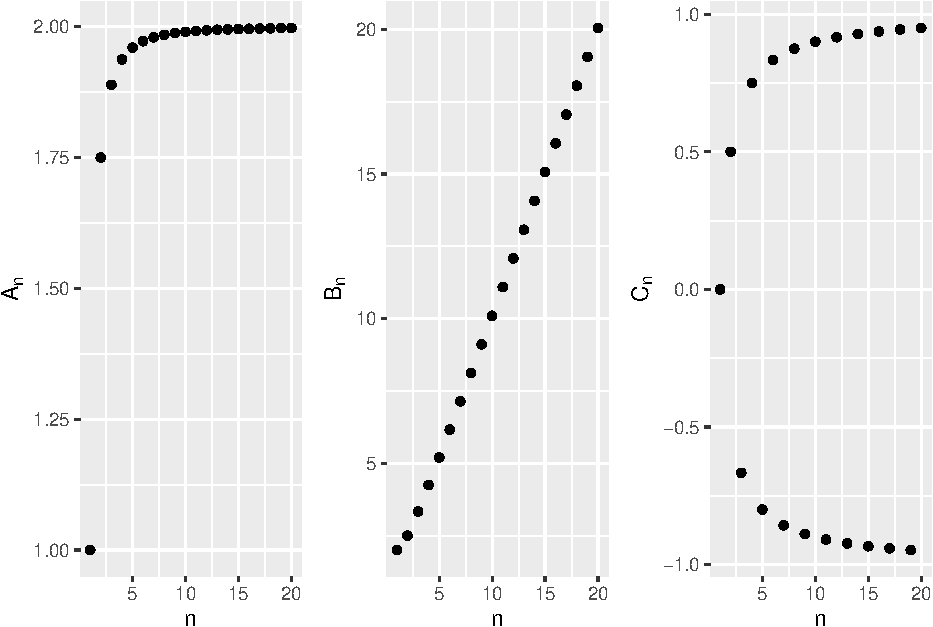
\includegraphics{figure-latex/seqabc-1.pdf}
\caption{\label{fig:seqabc}Behavior of Some Sequences}
\end{figure}

\hypertarget{the-limit-of-a-sequence}{%
\section{The Limit of a Sequence}\label{the-limit-of-a-sequence}}

The notion of ``converging to a limit'' is the behavior of the points in Example \ref{exm:seqbehav}. In some sense, that's the counterfactual we want to know. What happens as \(n\rightarrow \infty\)?

\begin{enumerate}
\def\labelenumi{\arabic{enumi}.}
\tightlist
\item
  Sequences like 1 above that converge to a limit.
\item
  Sequences like 2 above that increase without bound.
\item
  Sequences like 3 above that neither converge nor increase without bound --- alternating over the number line.
\end{enumerate}

\begin{definition}
\protect\hypertarget{def:unnamed-chunk-2}{}\label{def:unnamed-chunk-2}The sequence \(\{y_n\}\) has the limit \(L\), which we write as \[\lim\limits_{n \to \infty} y_n =L\], if for any \(\epsilon>0\) there is an integer \(N\) (which depends on \(\epsilon\)) with the property that \(|y_n -L|<\epsilon\) for each \(n>N\). \(\{y_n\}\) is said to converge to \(L\). If the above does not hold, then \(\{y_n\}\) diverges.
\end{definition}

We can also express the behavior of a sequence as bounded or not:

\begin{enumerate}
\def\labelenumi{\arabic{enumi}.}
\tightlist
\item
  Bounded: if \(|y_n|\le K\) for all \(n\)
\item
  Monotonically Increasing: \(y_{n+1}>y_n\) for all \(n\)
\item
  Monotonically Decreasing: \(y_{n+1}<y_n\) for all \(n\)
\end{enumerate}

A limit is \emph{unique}: If \(\{y_n\}\) converges, then the limit \(L\) is unique.

If a sequence converges, then the sum of such sequences also converges. Let \(\lim\limits_{n \to \infty} y_n = y\) and \(\lim\limits_{n \to \infty} z_n =z\). Then

\begin{enumerate}
\def\labelenumi{\arabic{enumi}.}
\tightlist
\item
  \(\lim\limits_{n \to \infty} [k y_n + \ell z_n]= k y + \ell z\)
\item
  \(\lim\limits_{n \to \infty} y_n z_n = yz\)
\item
  \(\lim\limits_{n \to \infty} \frac{y_n}{z_n} = \frac{y}{z}\), provided \(z\neq 0\)
\end{enumerate}

This looks reasonable enough. The harder question, obviously is when the parts of the fraction \emph{don't} converge. If \(\lim_{n\to\infty} y_n = \infty\) and \(\lim_{n\to\infty} z_n = \infty\), What is \(\lim_{n\to\infty} y_n - z_n\)? What is \(\lim_{n\to\infty} \frac{y_n}{z_n}\)?

It is nice for a sequence to converge in limit. We want to know if complex-looking sequences converge or not. The name of the game here is to break that complex sequence up into sums of simple fractions where \(n\) only appears in the denominator: \(\frac{1}{n}, \frac{1}{n^2}\), and so on. Each of these will converge to 0, because the denominator gets larger and larger. Then, because of the properties above, we can then find the final sequence.

\begin{example}[Simplifying a Fraction into Sums]
\protect\hypertarget{exm:unnamed-chunk-3}{}\label{exm:unnamed-chunk-3}Find the limit of
\[\lim_{n\to \infty} \frac{n + 3}{n},\]
\end{example}

\begin{solution}
At first glance, \(n + 3\) and \(n\) both grow to \(\infty\), so it looks like we need to divide infinity by infinity. However, we can express this fraction as a sum, then the limits apply separately:

\[\lim_{n\to \infty} \frac{n + 3}{n} = \lim_{n\to \infty} \left(1 + \frac{3}{n}\right) =  \underbrace{\lim_{n\to \infty}1}_{1} +  \underbrace{\lim_{n\to \infty}\left(\frac{3}{n}\right)}_{0}\]

so, the limit is actually 1.
\end{solution}

After some practice, the key to intuition is whether one part of the fraction grows ``faster'' than another. If the denominator grows faster to infinity than the numerator, then the fraction will converge to 0, even if the numerator will also increase to infinity. In a sense, limits show how not all infinities are the same.

\begin{exercise}
\protect\hypertarget{exr:limseq2}{}\label{exr:limseq2}

Find the following limits of sequences, then explain in English the intuition for why that is the case.

\begin{enumerate}
\def\labelenumi{\arabic{enumi}.}
\tightlist
\item
  \(\lim\limits_{n\to\infty} \frac{2n}{n^2 + 1}\)
\item
  \(\lim\limits_{n\to\infty} (n^3 - 100n^2)\)
\end{enumerate}

\end{exercise}

\hypertarget{limitsfun}{%
\section{Limits of a Function}\label{limitsfun}}

We've now covered functions and just covered limits of sequences, so now is the time to combine the two.

A function \(f\) is a compact representation of some behavior we care about. Like for sequences, we often want to know if \(f(x)\) approaches some number \(L\) as its independent variable \(x\) moves to some number \(c\) (which is usually 0 or \(\pm\infty\)). If it does, we say that the limit of \(f(x)\), as \(x\) approaches \(c\), is \(L\): \(\lim\limits_{x \to c} f(x)=L\). Unlike a sequence, \(x\) is a continuous number, and we can move in decreasing order as well as increasing.

For a limit \(L\) to exist, the function \(f(x)\) must approach \(L\) from both the left (increasing) and the right (decreasing).

\begin{definition}[Limit of a function]
\protect\hypertarget{def:unnamed-chunk-5}{}\label{def:unnamed-chunk-5}Let \(f(x)\) be defined at each point in some open interval containing the point \(c\). Then \(L\) equals \(\lim\limits_{x \to c} f(x)\) if for any (small positive) number \(\epsilon\), there exists a corresponding number \(\delta>0\) such that if \(0<|x-c|<\delta\), then \(|f(x)-L|<\epsilon\).
\end{definition}

A neat, if subtle result is that \(f(x)\) does not necessarily have to be defined at \(c\) for \(\lim\limits_{x \to c}\) to exist.

Properties: Let \(f\) and \(g\) be functions with \(\lim\limits_{x \to c} f(x)=k\) and \(\lim\limits_{x \to c} g(x)=\ell\).

\begin{enumerate}
\def\labelenumi{\arabic{enumi}.}
\tightlist
\item
  \(\lim\limits_{x \to c}[f(x)+g(x)]=\lim\limits_{x \to c} f(x)+ \lim\limits_{x \to c} g(x)\)
\item
  \(\lim\limits_{x \to c} kf(x) = k\lim\limits_{x \to c} f(x)\)
\item
  \(\lim\limits_{x \to c} f(x) g(x) = \left[\lim\limits_{x \to c} f(x)\right]\cdot \left[\lim\limits_{x \to c} g(x)\right]\)
\item
  \(\lim\limits_{x \to c} \frac{f(x)}{g(x)} = \frac{\lim\limits_{x \to c} f(x)}{\lim\limits_{x \to c} g(x)}\), provided \(\lim\limits_{x \to c} g(x)\ne 0\).
\end{enumerate}

Simple limits of functions can be solved as we did limits of sequences. Just be careful which part of the function is changing.

\begin{example}[Limits of Functions]
\protect\hypertarget{exm:limfun1}{}\label{exm:limfun1}

Find the limit of the following functions.

\begin{enumerate}
\def\labelenumi{\arabic{enumi}.}
\tightlist
\item
  \(\lim_{x \to c} k\)
\item
  \(\lim_{x \to c} x\)
\item
  \(\lim_{x\to 2} (2x-3)\)
\item
  \(\lim_{x \to c} x^n\)
\end{enumerate}

\end{example}

Limits can get more complex in roughly two ways. First, the functions may become large polynomials with many moving pieces. Second,the functions may become discontinuous.

The function can be thought of as a more general or ``smooth'' version of sequences. For example,

\begin{exercise}[Limits of a Fraction of Functions]
\protect\hypertarget{exr:limfunmax}{}\label{exr:limfunmax}Find the limit of

\[\lim_{x\to\infty} \frac{(x^4 +3x−99)(2−x^5)}{(18x^7 +9x^6 −3x^2 −1)(x+1)}\]
\end{exercise}

Now, the functions will become a bit more complex:

\begin{exercise}
\protect\hypertarget{exr:discontlim}{}\label{exr:discontlim}

Solve the following limits of functions

\begin{enumerate}
\def\labelenumi{\arabic{enumi}.}
\tightlist
\item
  \(\lim\limits_{x\to 0} |x|\)
\item
  \(\lim\limits_{x\to 0} \left(1+\frac{1}{x^2}\right)\)
\end{enumerate}

\end{exercise}

So there are a few more alternatives about what a limit of a function could be:

\begin{enumerate}
\def\labelenumi{\arabic{enumi}.}
\tightlist
\item
  Right-hand limit: The value approached by \(f(x)\) when you move from right to left.
\item
  Left-hand limit: The value approached by \(f(x)\) when you move from left to right.
\item
  Infinity: The value approached by \(f(x)\) as x grows infinitely large. Sometimes this may be a number; sometimes it might be \(\infty\) or \(-\infty\).
\item
  Negative infinity: The value approached by \(f(x)\) as x grows infinitely negative. Sometimes this may be a number; sometimes it might be \(\infty\) or \(-\infty\).
\end{enumerate}

The distinction between left and right becomes important when the function is not determined for some values of \(x\). What are those cases in the examples below?

\begin{figure}
\centering
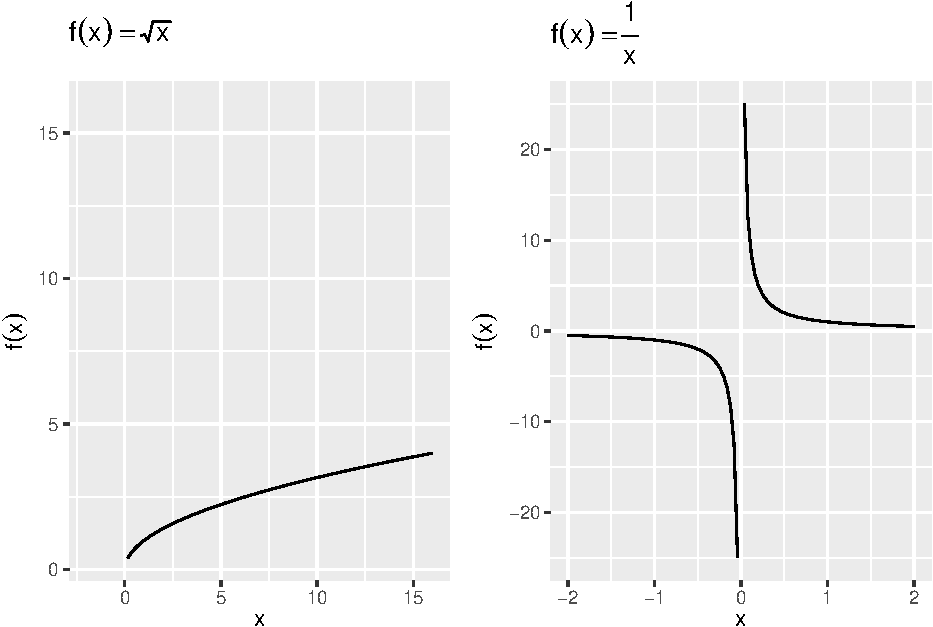
\includegraphics{figure-latex/unnamed-chunk-6-1.pdf}
\caption{\label{fig:unnamed-chunk-6}Functions which are not defined in some areas}
\end{figure}

\hypertarget{continuity}{%
\section{Continuity}\label{continuity}}

To repeat a finding from the limits of functions: \(f(x)\) does not necessarily have to be defined at \(c\) for \(\lim\limits_{x \to c}\) to exist. Functions that have breaks in their lines are called discontinuous. Functions that have no breaks are called continuous. Continuity is a concept that is more fundamental to, but related to that of ``differentiability'', which we will cover next in calculus.

\begin{definition}[Continuity]
\protect\hypertarget{def:unnamed-chunk-7}{}\label{def:unnamed-chunk-7}Suppose that the domain of the function \(f\) includes an open interval containing the point \(c\). Then \(f\) is continuous at \(c\) if \(\lim\limits_{x \to c} f(x)\) exists and if \(\lim\limits_{x \to c} f(x)=f(c)\). Further, \(f\) is continuous on an open interval \((a,b)\) if it is continuous at each point in the interval.
\end{definition}

To prove that a function is continuous for all points is beyond this practical introduction to math, but the general intuition can be grasped by graphing.

\begin{example}[Continuous and Discontinuous Functions]
\protect\hypertarget{exm:contdiscont}{}\label{exm:contdiscont}For each function, determine if it is continuous or discontinuous.

\begin{enumerate}
\def\labelenumi{\arabic{enumi}.}
\tightlist
\item
  \(f(x) = \sqrt{x}\)
\item
  \(f(x) = e^x\)
\item
  \(f(x) = 1 + \frac{1}{x^2}\)
\item
  \(f(x) = \text{floor}(x)\).
\end{enumerate}

The floor is the smaller of the two integers bounding a number. So \(\text{floor}(x = 2.999) = 2\), \(\text{floor}(x = 2.0001) = 2\), and \(\text{floor}(x = 2) = 2.\)
\end{example}

\begin{solution}
In Figure \ref{fig:fig-contdiscont}, we can see that the first two functions are continuous, and the next two are discontinuous. \(f(x) = 1 + \frac{1}{x^2}\) is discontinuous at \(x= 0\), and \(f(x) = \text{floor}(x)\) is discontinuous at each whole number.
\end{solution}

\begin{figure}
\centering
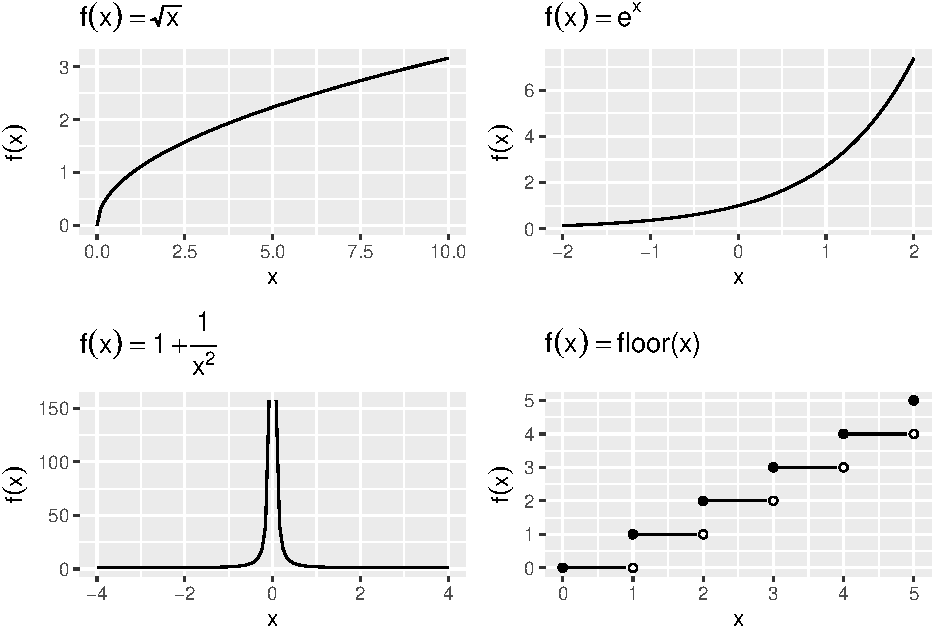
\includegraphics{figure-latex/fig-contdiscont-1.pdf}
\caption{\label{fig:fig-contdiscont}Continuous and Discontinuous Functions}
\end{figure}

Some properties of continuous functions:

\begin{enumerate}
\def\labelenumi{\arabic{enumi}.}
\tightlist
\item
  If \(f\) and \(g\) are continuous at point \(c\), then \(f+g\), \(f-g\), \(f \cdot g\), \(|f|\), and \(\alpha f\) are continuous at point \(c\) also. \(f/g\) is continuous, provided \(g(c)\ne 0\).
\item
  Boundedness: If \(f\) is continuous on the closed bounded interval \([a,b]\), then there is a number \(K\) such that \(|f(x)|\le K\) for each \(x\) in \([a,b]\).
\item
  Max/Min: If \(f\) is continuous on the closed bounded interval \([a,b]\), then \(f\) has a maximum and a minimum on \([a,b]\). They may be located at the end points.
\end{enumerate}

\begin{exercise}[Limit when Denominator converges to 0]
\protect\hypertarget{exr:discontdraw}{}\label{exr:discontdraw}

Let \[f(x) = \frac{x^2 + 2x}{x}.\]

\begin{enumerate}
\def\labelenumi{\arabic{enumi}.}
\tightlist
\item
  Graph the function. Is it defined everywhere?
\item
  What is the functions limit at \(x \rightarrow 0\)?
\end{enumerate}

\end{exercise}


\hypertarget{example-the-central-limit-theorem}{%
\section*{Example: The Central Limit Theorem}\label{example-the-central-limit-theorem}}
\addcontentsline{toc}{section}{Example: The Central Limit Theorem}

Perhaps the most important theorem in statistics is the Central Limit Theorem,

\begin{theorem}[Central Limit Theorem (i.i.d. case)]
\protect\hypertarget{thm:clt-lim}{}\label{thm:clt-lim}For any series of independent and identically distributed random variables \(X_1, X_2, \cdots\), we know the distribution of its sum even if we do not know the distribution of \(X\). The distribution of the sum is a Normal distribution.

\[\frac{\bar{X}_n - \mu}{\sigma / \sqrt{n}} \xrightarrow{d} \text{Normal}(0, 1),\]

where \(\mu\) is the mean of \(X\) and \(\sigma\) is the standard deviation of \(X\). The arrow is read as ``converges in distribution to''. \(\text{Normal}(0, 1)\) indicates a Normal Distribution with mean 0 and variance 1.

That is, the limit of the distribution of the lefthand side is the distribution of the righthand side.
\end{theorem}

The sign of a limit is the arrow ``\(\rightarrow\)''. Although we have not yet covered probability (in Section \ref{probability-theory}) so we have not described what distributions and random variables are, it is worth foreshadowing the Central Limit Theorem. The Central Limit Theorem is powerful because it gives us a \emph{guarantee} of what would happen if \(n \rightarrow \infty\), which in this case means we collected more data.

\hypertarget{example-the-law-of-large-numbers}{%
\section*{Example: The Law of Large Numbers}\label{example-the-law-of-large-numbers}}
\addcontentsline{toc}{section}{Example: The Law of Large Numbers}

A finding that perhaps rivals the Central Limit Theorem is the Law of Large Numbers:

\begin{theorem}[(Weak) Law of Large Numbers]
\protect\hypertarget{thm:lln-lim}{}\label{thm:lln-lim}For any draw of identically distributed independent variables with mean \(\mu\), the sample average after \(n\) draws, \(\bar{X}_n\), converges in probability to the true mean as \(n \rightarrow \infty\):

\[\lim\limits_{n\to \infty} P(|\bar{X}_n - \mu | > \varepsilon) = 0\]

A shorthand of which is \(\bar{X}_n \xrightarrow{p} \mu\), where the arrow is read as ``converges in probability to''.
\end{theorem}

Intuitively, the more data, the more accurate is your guess. For example, the Figure \ref{fig:llnsim} shows how the sample average from many coin tosses converges to the true value : 0.5.

\begin{figure}
\centering
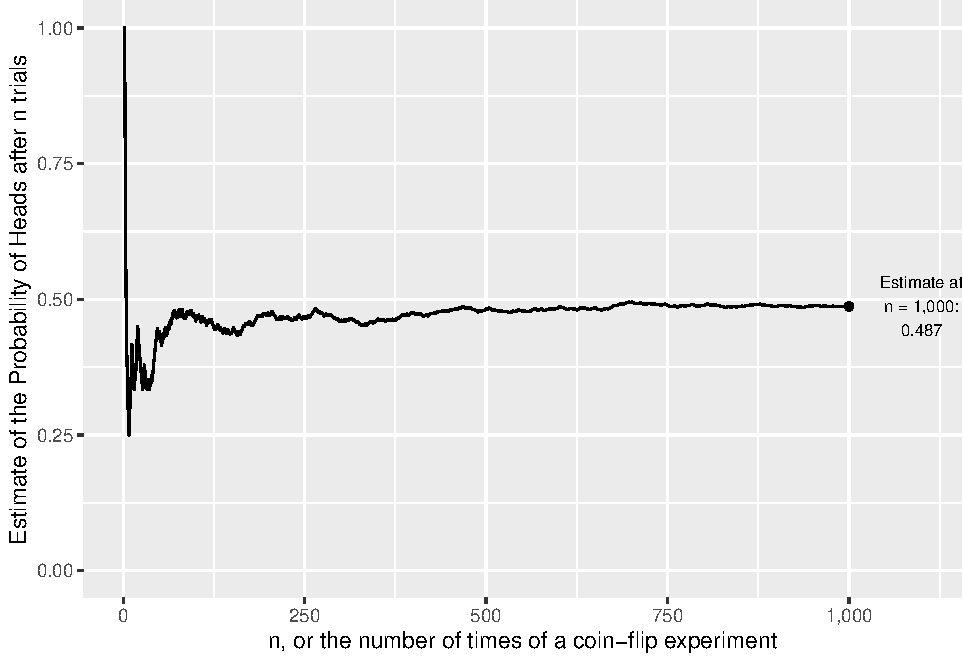
\includegraphics{figure-latex/llnsim-1.pdf}
\caption{\label{fig:llnsim}As the number of coin tosses goes to infinity, the average probabiity of heads converges to 0.5}
\end{figure}


\hypertarget{derivatives}{%
\chapter{Calculus}\label{derivatives}}

Calculus is a fundamental part of any type of statistics exercise. Although you may not be taking derivatives and integral in your daily work as an analyst, calculus undergirds many concepts we use: maximization, expectation, and cumulative probability.

\hypertarget{derivintro}{%
\section{Derivatives}\label{derivintro}}

The derivative of \(f\) at \(x\) is its rate of change at \(x\): how much \(f(x)\) changes with a change in \(x\). The rate of change is a fraction --- rise over run --- but because not all lines are straight and the rise over run formula will give us different values depending on the range we examine, we need to take a limit (Section \ref{limits-precalc}).

\begin{definition}[Derivative]
\protect\hypertarget{def:unnamed-chunk-15}{}\label{def:unnamed-chunk-15}

Let \(f\) be a function whose domain includes an open interval containing the point \(x\). The derivative of \(f\) at \(x\) is given by

\[\frac{d}{dx}f(x) =\lim\limits_{h\to 0} \frac{f(x+h)-f(x)}{(x+h)-x} = \lim\limits_{h\to 0} \frac{f(x+h)-f(x)}{h}
\]

There are a two main ways to denote a derivate:

\begin{itemize}
\tightlist
\item
  Leibniz Notation: \(\frac{d}{dx}(f(x))\)
\item
  Prime or Lagrange Notation: \(f'(x)\)
\end{itemize}

\end{definition}

If \(f(x)\) is a straight line, the derivative is the slope. For a curve, the slope changes by the values of \(x\), so the derivative is the slope of the line tangent to the curve at \(x\). See, For example, Figure \ref{fig:derivsimple}.

\begin{figure}
\centering
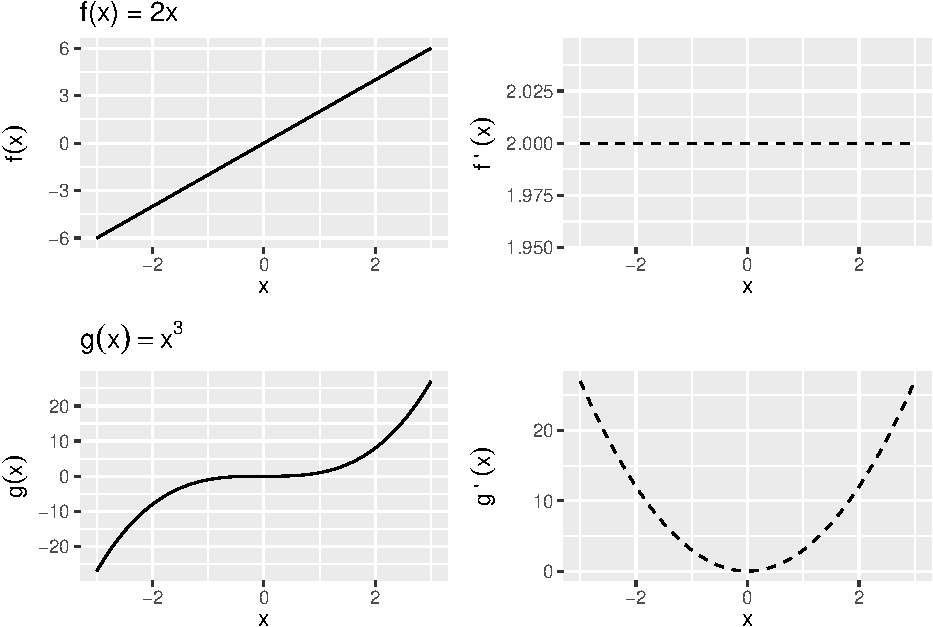
\includegraphics{figure-latex/derivsimple-1.pdf}
\caption{\label{fig:derivsimple}The Derivative as a Slope}
\end{figure}

If \(f'(x)\) exists at a point \(x_0\), then \(f\) is said to be \textbf{differentiable} at \(x_0\). That also implies that \(f(x)\) is continuous at \(x_0\).

\hypertarget{properties-of-derivatives}{%
\subsection*{Properties of derivatives}\label{properties-of-derivatives}}
\addcontentsline{toc}{subsection}{Properties of derivatives}

Suppose that \(f\) and \(g\) are differentiable at \(x\) and that \(\alpha\) is a constant. Then the functions \(f\pm g\), \(\alpha f\), \(f g\), and \(f/g\) (provided \(g(x)\ne 0\)) are also differentiable at \(x\). Additionally,

\textbf{Constant rule:} \[\left[k f(x)\right]' = k f'(x)\]

\textbf{Sum rule:} \[\left[f(x)\pm g(x)\right]' = f'(x)\pm g'(x)\]

With a bit more algebra, we can apply the definition of derivatives to get a formula for of the derivative of a product and a derivative of a quotient.

\textbf{Product rule:} \[\left[f(x)g(x)\right]^\prime = f^\prime(x)g(x)+f(x)g^\prime(x)\]

\textbf{Quotient rule:} \[\left[f(x)/g(x)\right]^\prime = \frac{f^\prime(x)g(x) - f(x)g^\prime(x)}{[g(x)]^2}, ~g(x)\neq 0\]

Finally, one way to think of the power of derivatives is that it takes a function a notch down in complexity. The power rule applies to any higher-order function:

\textbf{Power rule:} \[\left[x^k\right]^\prime = k x^{k-1}\]

For any real number \(k\) (that is, both whole numbers and fractions). The power rule is proved \textbf{by induction}, a neat method of proof used in many fundamental applications to prove that a general statement holds for every possible case, even if there are countably infinite cases. We'll show a simple case where \(k\) is an integer here.

\begin{proof}[Proof of Power Rule by Induction]
We would like to prove that

\[\left[x^k\right]^\prime = k x^{k-1}\]
for any integer \(k\).

First, consider the first case (the base case) of \(k = 1\). We can show by the definition of derivatives (setting \(f(x) = x^1 = 1\)) that

\[[x^1]^\prime = \lim_{h \rightarrow 0}\frac{(x + h) - x}{(x + h) - x}= 1.\]

Because \(1\) is also expressed as \(1 x^{1- 1}\), the statement we want to prove holds for the case \(k =1\).

Now, \emph{assume} that the statement holds for some integer \(m\). That is, assume
\[\left[x^m\right]^\prime = m x^{m-1}\]

Then, for the case \(m + 1\), using the product rule above, we can simplify

\begin{align*}
\left[x^{m + 1}\right]^\prime &= [x^{m}\cdot x]^\prime\\
&= (x^m)^\prime\cdot x + (x^m)\cdot (x)^\prime\\
&= m x^{m - 1}\cdot x + x^m ~~\because \text{by previous assumption}\\
&= mx^m + x^m\\
&= (m + 1)x^m\\
&= (m + 1)x^{(m + 1) - 1}
\end{align*}

Therefore, the rule holds for the case \(k = m + 1\) once we have assumed it holds for \(k = m\). Combined with the first case, this completes proof by induction -- we have now proved that the statement holds for all integers \(k = 1, 2, 3, \cdots\).

To show that it holds for real fractions as well, we can prove expressing that exponent by a fraction of two integers.
\end{proof}

These ``rules'' become apparent by applying the definition of the derivative above to each of the things to be ``derived'', but these come up so frequently that it is best to repeat until it is muscle memory.

\begin{exercise}[Derivative of Polynomials]
\protect\hypertarget{exr:introderivatives}{}\label{exr:introderivatives}

For each of the following functions, find the first-order derivative \(f^\prime(x)\).

\begin{enumerate}
\def\labelenumi{\arabic{enumi}.}
\tightlist
\item
  \(f(x)=c\)
\item
  \(f(x)=x\)
\item
  \(f(x)=x^2\)
\item
  \(f(x)=x^3\)
\item
  \(f(x)=\frac{1}{x^2}\)
\item
  \(f(x)=(x^3)(2x^4)\)
\item
  \(f(x) = x^4 - x^3 + x^2 - x + 1\)
\item
  \(f(x) = (x^2 + 1)(x^3 - 1)\)
\item
  \(f(x) = 3x^2 + 2x^{1/3}\)
\item
  \(f(x)=\frac{x^2+1}{x^2-1}\)
\end{enumerate}

\end{exercise}

\hypertarget{derivpoly}{%
\section{Higher-Order Derivatives (Derivatives of Derivatives of Derivatives)}\label{derivpoly}}

The first derivative is applying the definition of derivatives on the function, and it can be expressed as

\[f'(x),  ~~ y',  ~~ \frac{d}{dx}f(x), ~~ \frac{dy}{dx}\]

We can keep applying the differentiation process to functions that are themselves derivatives. The derivative of \(f'(x)\) with respect to \(x\), would then be \[f''(x)=\lim\limits_{h\to 0}\frac{f'(x+h)-f'(x)}{h}\] and we can therefore call it the \textbf{Second derivative:}

\[f''(x), ~~ y'', ~~ \frac{d^2}{dx^2}f(x), ~~ \frac{d^2y}{dx^2}\]

Similarly, the derivative of \(f''(x)\) would be called the third derivative and is denoted \(f'''(x)\). And by extension, the \textbf{nth derivative} is expressed as \(\frac{d^n}{dx^n}f(x)\), \(\frac{d^ny}{dx^n}\).

\begin{example}[Succession of Derivatives]
\protect\hypertarget{exm:unnamed-chunk-16}{}\label{exm:unnamed-chunk-16}\begin{align*}
f(x) &=x^3\\
f^{\prime}(x) &=3x^2\\
f^{\prime\prime}(x) &=6x \\
f^{\prime\prime\prime}(x) &=6\\
f^{\prime\prime\prime\prime}(x) &=0\\
\end{align*}
\end{example}

Earlier, in Section \ref{derivintro}, we said that if a function differentiable at a given point, then it must be continuous. Further, if \(f'(x)\) is itself continuous, then \(f(x)\) is called continuously differentiable. All of this matters because many of our findings about optimization (Section \ref{optim}) rely on differentiation, and so we want our function to be differentiable in as many layers. A function that is continuously differentiable infinitly is called ``smooth''. Some examples: \(f(x) = x^2\), \(f(x) = e^x\).

\hypertarget{composite-functions-and-the-chain-rule}{%
\section{Composite Functions and the Chain Rule}\label{composite-functions-and-the-chain-rule}}

As useful as the above rules are, many functions you'll see won't fit neatly in each case immediately. Instead, they will be functions of functions. For example, the difference between \(x^2 + 1^2\) and \((x^2 + 1)^2\) may look trivial, but the sum rule can be easily applied to the former, while it's actually not obvious what do with the latter.

\textbf{Composite functions} are formed by substituting one function into another and are denoted by \[(f\circ g)(x)=f[g(x)].\] To form \(f[g(x)]\), the range of \(g\) must be contained (at least in part) within the domain of \(f\). The domain of \(f\circ g\) consists of all the points in the domain of \(g\) for which \(g(x)\) is in the domain of \(f\).

\begin{example}
\protect\hypertarget{exm:unnamed-chunk-17}{}\label{exm:unnamed-chunk-17}Let \(f(x)=\log x\) for \(0<x<\infty\) and \(g(x)=x^2\) for \(-\infty<x<\infty\).

Then
\[(f\circ g)(x)=\log x^2, -\infty<x<\infty - \{0\}\]

Also
\[(g\circ f)(x)=[\log x]^2, 0<x<\infty\]

Notice that \(f\circ g\) and \(g\circ f\) are not the same functions.
\end{example}

With the notation of composite functions in place, now we can introduce a helpful additional rule that will deal with a derivative of composite functions as a chain of concentric derivatives.

\textbf{Chain Rule}:

Let \(y=(f\circ g)(x)= f[g(x)]\). The derivative of \(y\) with respect to \(x\) is \[\frac{d}{dx} \{ f[g(x)] \} = f'[g(x)] g'(x)\]

We can read this as: ``the derivative of the composite function \(y\) is the derivative of \(f\) evaluated at \(g(x)\), times the derivative of \(g\).''

The chain rule can be thought of as the derivative of the ``outside'' times the derivative of the ``inside'', remembering that the derivative of the outside function is evaluated at the value of the inside function.

\begin{itemize}
\tightlist
\item
  The chain rule can also be written as \[\frac{dy}{dx}=\frac{dy}{dg(x)} \frac{dg(x)}{dx}\] This expression does not imply that the \(dg(x)\)'s cancel out, as in fractions. They are part of the derivative notation and you can't separate them out or cancel them.)
\end{itemize}

\begin{example}[Composite Exponent]
\protect\hypertarget{exm:tothesix}{}\label{exm:tothesix}Find \(f^\prime(x)\) for \(f(x) = (3x^2+5x-7)^6\).
\end{example}

The direct use of a chain rule is when the exponent of is itself a function, so the power rule could not have applied generaly:

\textbf{Generalized Power Rule}:

If \(f(x)=[g(x)]^p\) for any rational number \(p\), \[f^\prime(x) =p[g(x)]^{p-1}g^\prime(x)\]

\hypertarget{derivatives-of-natural-logs-and-the-exponent}{%
\section{Derivatives of natural logs and the exponent}\label{derivatives-of-natural-logs-and-the-exponent}}

Natural logs and exponents (they are inverses of each other; see Section \ref{logexponents}) crop up everywhere in statistics. Their derivative is a special case from the above, but quite elegant.

\begin{theorem}
\protect\hypertarget{thm:derivexplog}{}\label{thm:derivexplog}The functions \(e^x\) and the natural logarithm \(\log(x)\) are continuous and differentiable in their domains, and their first derivate is
\[(e^x)^\prime = e^x\]
\[\log(x)^\prime = \frac{1}{x}\]

Also, when these are composite functions, it follows by the generalized power rule that

\[\left(e^{g(x)}\right)^\prime = e^{g(x)} \cdot g^\prime(x)\]
\[\left(\log g(x)\right)^\prime = \frac{g^\prime(x)}{g(x)}, ~~\text{if}~~ g(x) > 0\]
\end{theorem}

We will relegate the proofs to small excerpts.

\hypertarget{derivatives-of-natural-exponential-function-e}{%
\subsection*{\texorpdfstring{Derivatives of natural exponential function (\(e\))}{Derivatives of natural exponential function (e)}}\label{derivatives-of-natural-exponential-function-e}}
\addcontentsline{toc}{subsection}{Derivatives of natural exponential function (\(e\))}

To repeat the main rule in Theorem \ref{thm:derivexplog}, the intuition is that

\begin{enumerate}
\def\labelenumi{\arabic{enumi}.}
\tightlist
\item
  Derivative of \(e^x\) is itself: \(\frac{d}{dx}e^x = e^x\) (See Figure \ref{fig:fig-derivexponent})
\item
  Same thing if there were a constant in front: \(\frac{d}{dx}\alpha e^x = \alpha e^x\)
\item
  Same thing no matter how many derivatives there are in front: \(\frac{d^n}{dx^n} \alpha e^x = \alpha e^x\)
\item
  Chain Rule: When the exponent is a function of \(x\), remember to take derivative of that function and add to product. \(\frac{d}{dx}e^{g(x)}= e^{g(x)} g^\prime(x)\)
\end{enumerate}

\begin{figure}
\centering
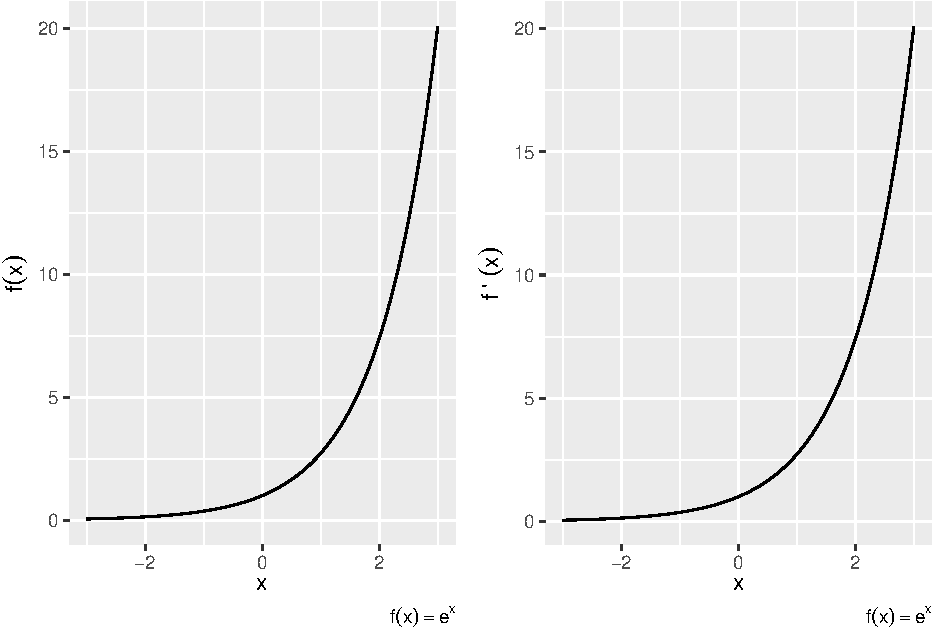
\includegraphics{figure-latex/fig-derivexponent-1.pdf}
\caption{\label{fig:fig-derivexponent}Derivative of the Exponential Function}
\end{figure}

\begin{example}[Derivative of exponents]
\protect\hypertarget{exm:exmderivexp}{}\label{exm:exmderivexp}

Find the derivative for the following.

\begin{enumerate}
\def\labelenumi{\arabic{enumi}.}
\tightlist
\item
  \(f(x)=e^{-3x}\)
\item
  \(f(x)=e^{x^2}\)
\item
  \(f(x)=(x-1)e^x\)
\end{enumerate}

\end{example}

\hypertarget{derivatives-of-log}{%
\subsection*{\texorpdfstring{Derivatives of \(\log\)}{Derivatives of \textbackslash log}}\label{derivatives-of-log}}
\addcontentsline{toc}{subsection}{Derivatives of \(\log\)}

The natural log is the mirror image of the natural exponent and has mirroring properties, again, to repeat the theorem,

\begin{enumerate}
\def\labelenumi{\arabic{enumi}.}
\tightlist
\item
  log prime x is one over x: \(\frac{d}{dx} \log x = \frac{1}{x}\) (Figure \ref{fig:fig-derivlog})
\item
  Exponents become multiplicative constants: \(\frac{d}{dx} \log x^k = \frac{d}{dx} k \log x = \frac{k}{x}\)
\item
  Chain rule again: \(\frac{d}{dx} \log u(x) = \frac{u'(x)}{u(x)}\quad\)
\item
  For any positive base \(b\), \(\frac{d}{dx} b^x = (\log b)\left(b^x\right)\).
\end{enumerate}

\begin{figure}
\centering
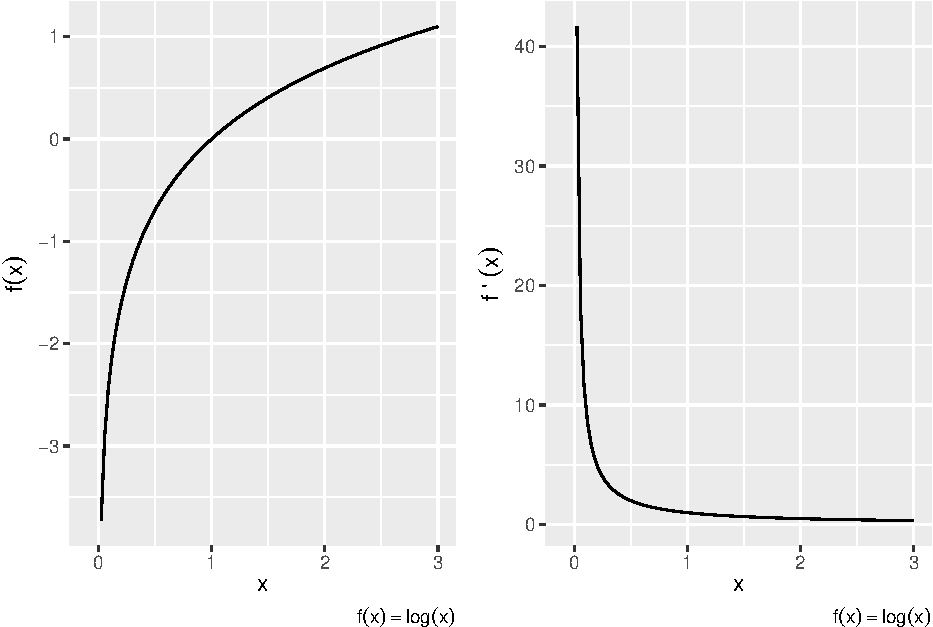
\includegraphics{figure-latex/fig-derivlog-1.pdf}
\caption{\label{fig:fig-derivlog}Derivative of the Natural Log}
\end{figure}

\begin{example}[Derivative of logs]
\protect\hypertarget{exm:exmderivlog}{}\label{exm:exmderivlog}

Find \(dy/dx\) for the following.

\begin{enumerate}
\def\labelenumi{\arabic{enumi}.}
\tightlist
\item
  \(f(x)=\log(x^2+9)\)
\item
  \(f(x)=\log(\log x)\)
\item
  \(f(x)=(\log x)^2\)
\item
  \(f(x)=\log e^x\)
\end{enumerate}

\end{example}

\hypertarget{outline-of-proof}{%
\subsection*{Outline of Proof}\label{outline-of-proof}}
\addcontentsline{toc}{subsection}{Outline of Proof}

We actually show the derivative of the log first, and then the derivative of the exponential naturally follows.

The general derivative of the log at any base \(a\) is solvable by the definition of derivatives.

\begin{align*}
(\log_a x)^\prime = \lim\limits_{h\to 0} \frac{1}{h}\log_{a}\left(1 + \frac{h}{x}\right)
\end{align*}

Re-express \(g = \frac{h}{x}\) and get
\begin{align*}
(\log_a x)^\prime &= \frac{1}{x}\lim_{g\to 0}\log_{a} (1 + g)^{\frac{1}{g}}\\
&= \frac{1}{x}\log_a e
\end{align*}

By definition of \(e\). As a special case, when \(a = e\), then \((\log x)^\prime = \frac{1}{x}\).

Now let's think about the inverse, taking the derivative of \(y = a^x\).

\begin{align*}
y &= a^x \\
\Rightarrow \log y &= x \log a\\
\Rightarrow \frac{y^\prime}{y} &= \log a\\
\Rightarrow  y^\prime = y \log a\\
\end{align*}

Then in the special case where \(a = e\),

\[(e^x)^\prime = (e^x)\]

\hypertarget{partial-derivatives}{%
\section{Partial Derivatives}\label{partial-derivatives}}

What happens when there's more than variable that is changing?

\begin{quote}
If you can do ordinary derivatives, you can do partial derivatives: just hold all the other input variables constant except for the one you're differentiating with respect to. (Joe Blitzstein's Math Notes)
\end{quote}

Suppose we have a function \(f\) now of two (or more) variables and we want to determine the rate of change relative to one of the variables. To do so, we would find its partial derivative, which is defined similar to the derivative of a function of one variable.

\textbf{Partial Derivative}: Let \(f\) be a function of the variables \((x_1,\ldots,x_n)\). The partial derivative of \(f\) with respect to \(x_i\) is

\[\frac{\partial f}{\partial x_i} (x_1,\ldots,x_n) = \lim\limits_{h\to 0} \frac{f(x_1,\ldots,x_i+h,\ldots,x_n)-f(x_1,\ldots,x_i,\ldots,x_n)}{h}\]

Only the \(i\)th variable changes --- the others are treated as constants.

We can take higher-order partial derivatives, like we did with functions of a single variable, except now the higher-order partials can be with respect to multiple variables.

\begin{example}[More than one type of partial]
\protect\hypertarget{exm:unnamed-chunk-18}{}\label{exm:unnamed-chunk-18}Notice that you can take partials with regard to different variables.

Suppose \(f(x,y)=x^2+y^2\). Then

\begin{align*}
\frac{\partial f}{\partial x}(x,y) &=\\
\frac{\partial f}{\partial y}(x,y) &=\\
\frac{\partial^2 f}{\partial x^2}(x,y) &=\\
\frac{\partial^2 f}{\partial x \partial y}(x,y) &=
\end{align*}
\end{example}

\begin{exercise}
\protect\hypertarget{exr:unnamed-chunk-19}{}\label{exr:unnamed-chunk-19}Let \(f(x,y)=x^3 y^4 +e^x -\log y\). What are the following partial derivaitves?

\begin{align*}
\frac{\partial f}{\partial x}(x,y) &=\\
\frac{\partial f}{\partial y}(x,y) &=\\
\frac{\partial^2 f}{\partial x^2}(x,y) &=\\
\frac{\partial^2 f}{\partial x \partial y}(x,y) &= 
\end{align*}
\end{exercise}

\hypertarget{taylorapprox}{%
\section{Taylor Series Approximation}\label{taylorapprox}}

A common form of approximation used in statistics involves derivatives. A Taylor series is a way to represent common functions as infinite series (a sum of infinite elements) of the function's derivatives at some point \(a\).

For example, Taylor series are very helpful in representing nonlinear (read: difficult) functions as linear (read: manageable) functions. One can thus \textbf{approximate} functions by using lower-order, finite series known as \textbf{Taylor polynomials}. If \(a=0\), the series is called a Maclaurin series.

Specifically, a Taylor series of a real or complex function \(f(x)\) that is infinitely differentiable in the neighborhood of point \(a\) is:

\begin{align*}
    f(x) &= f(a) + \frac{f'(a)}{1!} (x-a) +  \frac{f''(a)}{2!} (x-a)^2 + \cdots\\
     &= \sum_{n=0}^\infty \frac{f^{(n)} (a)}{n!} (x-a)^n
\end{align*}

\textbf{Taylor Approximation}: We can often approximate the curvature of a function \(f(x)\) at point \(a\) using a 2nd order Taylor polynomial around point \(a\):

\[f(x) = f(a) + \frac{f'(a)}{1!} (x-a) +  \frac{f''(a)}{2!} (x-a)^2
+ R_2\]

\(R_2\) is the remainder (R for remainder, 2 for the fact that we took two derivatives) and often treated as negligible,
giving us:

\[f(x) \approx f(a) + f'(a)(x-a) +  \dfrac{f''(a)}{2} (x-a)^2\]

The more derivatives that are added, the smaller the remainder \(R\) and the more accurate the approximation. Proofs involving limits guarantee that the remainder converges to 0 as the order of derivation increases.

\end{document}
